\documentclass[11pt, a4paper]{article}
\usepackage{fullpage, mathpazo, microtype, parskip, graphicx}
\usepackage[no-weekday]{eukdate}
\usepackage[style=apa, terseinits=true, backend=biber, natbib=true, sorting=ynt, url=false, doi=false]{biblatex}
\defbibenvironment{bibliography}{\enumerate}{\endenumerate}{\item}
\defbibfilter{other}{not type=book and not type=thesis}
\bibliography{Gardner}


\begin{document}
\title{Obituary: Everette S Gardner Jr}
\author{Robert Fildes, Rob J Hyndman}
\maketitle

\begin{figure}[!ht]\centering
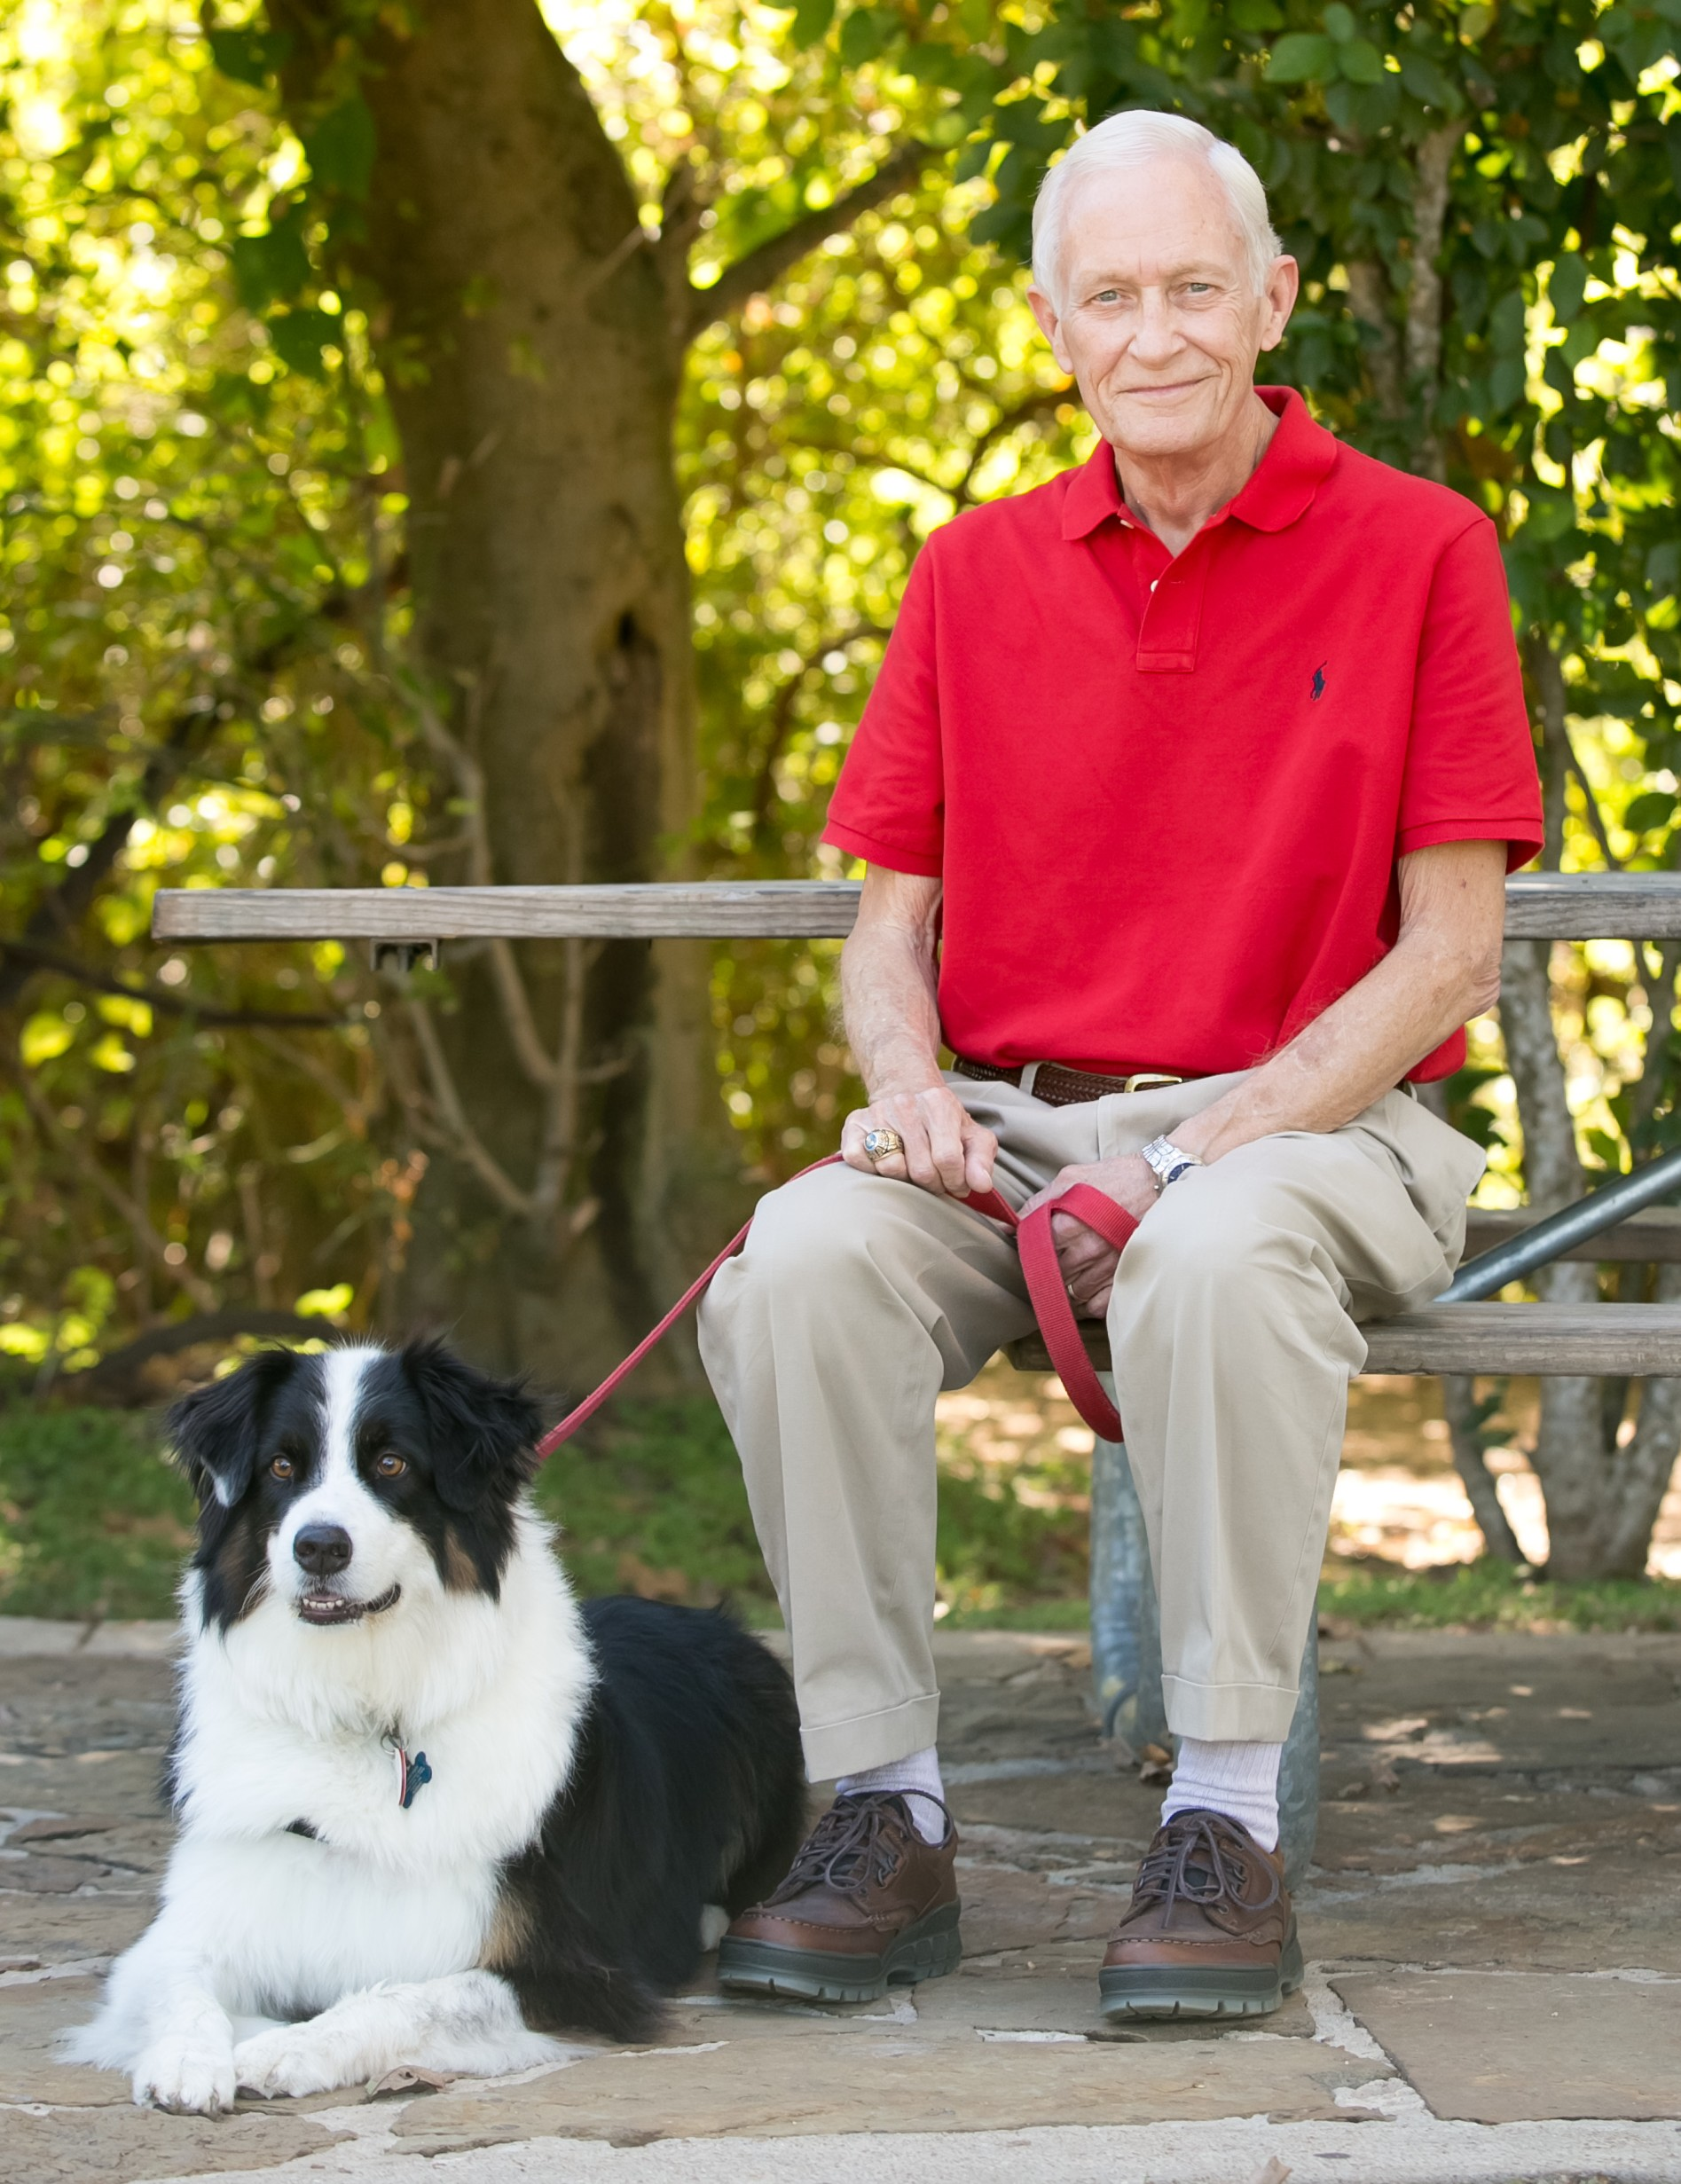
\includegraphics[width=7cm]{Ev_pic.jpg}
\centerline{\itshape Reproduced with permission from the University of Houston.}
\end{figure}

Everette ``Ev'' Gardner, Jr., a stalwart of the forecasting community for many years, died on 10\textsuperscript{th} September 2023, some 79 years after his birth in Arkansas. He graduated in 1966 from Memphis State University and immediately joined the US Navy. His Navy years proved critical in laying the foundations of his subsequent academic career, with sponsorship for an MBA and then, in 1976, a PhD \citep{phd} at the University of North Carolina, Chapel Hill. Ev's military experiences, including the undoubtedly onerous task of logistics manager for the Vietnam evacuation, were formative in influencing his approach to research, blending the practical challenges on the ground with rigour. His roles within operations, managing inventory for the USS Eisenhower, and Management Information Systems director for the US Atlantic Fleet, culminated in the position of Commander when he retired in 1986, at age 42.

In 1987, Ev joined the Department of Decision and Information Sciences, University of  Houston, Texas, and was quickly appointed chair and full professor. He remained there for the rest of his life, winning several awards for both his teaching and his research.

Ev's responsibilities and experiences in the Navy provided him with case studies which required the integration of two important areas of operations research, inventory control and forecasting, and it is here that his academic contributions arose. These two areas were (and still are) often treated discretely. His early career was marked by his appointment as associate editor of the \emph{Journal of Forecasting} (1983) and the \emph{International Journal of Forecasting} (1985), \emph{Management Science} (1987) and \emph{Interfaces} (1987), all highlighting this unusual mix of an expert practitioner who also had strong research interests. His authority, perhaps because of his naval background, led him to the board of the International Institute of Forecasters and its presidency in 1990. In 2007, Ev was elected a Fellow of the International Institute of Forecasters. He was a featured speaker at the International Symposium of Forecasting held in Prague, 2011, where his topic was ``Forecasting for Operations''.

His twin research interests led to a number of influential publications. In forecasting, he was particularly interested in exponential smoothing methods, which had their genesis in the US Navy in tracking submarines, and in forecasting the demand for spare parts in Navy inventory systems. Along with Eddie McKenzie from the University of Strathclyde, Ev proposed damped trend methods \citep{Gardner1985-lk,Gardner1989-bi}, which have since become an indispensable part of the exponential smoothing framework. Their argument was that trends are unlikely to continue unabated, and that longer-term forecasts are often more accurate when trends are damped or ignored.

His most cited works are the two "state of the art" papers \citep{Gardner1985-yu,Gardner2006-qq}, which expertly surveyed the literature on exponential smoothing at the time. In 2006, the first of these was ranked the third most influential article on forecasting by the International Institute of Forecasters. The second survey paper is still a great starting point for researchers interested in the area.

At the interface with inventory control, one of his most influential articles is \citet{Gardner1990-pw}, a case study based on his US Navy experience which shows how an  improved forecasting system, using his new damped trend method, paid off with both improved accuracy, but more importantly, improvements over the inventory investment/service tradeoff curve. We have both long regarded the problem formulation as fundamental to answering the question, ``is forecasting accuracy important?''. So much of the work in the area has pursued forecast accuracy without regard to costs or practical relevance. Ev pursued the same themes in the general context of global supply chains with his doctoral student, Yavuz Acar, in \citet{Acar2012ForecastingMS}. This was the first paper to show how to minimize total supply chain costs, taking account of the effects of forecast accuracy.

Throughout his career, Ev argued for using models with only the requisite complexity, and he presented these ideas in \citet{Syntetos2015ForecastingII}. Again, they showed that simple parametric methods performed well compared to more computationally demanding alternatives.

Ev took a keen interest in forecasting software, and developed his own spreadsheet-based software to do forecasting based on exponential smoothing, which he used in his extensive consulting activities. He also developed scheduling tools for spreadsheets, and both his forecasting and scheduling software were widely used for over a decade. In addition, he wrote three textbooks, based on using spreadsheets for managers \citep{book92,book93,book94}, along with co-authoring a more general book on quantitative methods in management \citep{book95}.

He was a committed teacher and a major contributor to the University of Houston Business Administration Honors program. All these activities were part of his vision of integrating research with practice, of which he was a tireless advocate in his publications, his consulting practice, and his teaching.

Sadly, he leaves a wife, Mary Ann, two children and their families, and his much-loved Australian Shepherd, Luke, who is a therapy dog visiting patients in the Houston area. Ev Gardner will be much missed, both professionally and personally.


\printbibliography

%\printbibliography[heading=subbibliography, title = {PhD}, type=thesis]
%\printbibliography[heading=subbibliography, title = {Books}, type=book]
%\printbibliography[heading=subbibliography, title = {Articles}, filter=other]

\end{document}
